\documentclass[conference]{IEEEtran}
\usepackage{amsmath,amssymb}
\usepackage{graphicx}
\usepackage{booktabs}
\usepackage{xcolor}
\usepackage{tikz}
\usetikzlibrary{arrows.meta,positioning}
\usepackage{url}

% Start a new row of author blocks (IEEEtran puts all authors in one row by default).
\makeatletter
\newcommand{\linebreakand}{\end{@IEEEauthorhalign}\hfill\mbox{}\par\mbox{}\hfill\begin{@IEEEauthorhalign}}
\makeatother

% Visible placeholder for results that do not exist yet or decisions the authors must make.
\newcommand{\todo}[1]{\textcolor{red}{\textbf{[TODO: #1]}}}

\begin{document}

\title{Reading Analog Gauges from Oblique Photographs:\\A Controlled Comparison of Tilt-Correction Strategies%
\thanks{Course project for CS4231 Fundamentals of Computer Vision, RV University, under the guidance of
Prof.\ Dr.~Ramakrishnan Varadharajan.}}

\author{%
\IEEEauthorblockN{Samarth Pyati}
\IEEEauthorblockA{1RVU23CSE400\\School of Computer Science and Engineering (SoCSE)\\RV University, Bengaluru, India\\samarthsp.btech23@rvu.edu.in}
\and
\IEEEauthorblockN{Amit Narendra}
\IEEEauthorblockA{1RVU23CSE042\\School of Computer Science and Engineering (SoCSE)\\RV University, Bengaluru, India\\amitcnarendra.btech23@rvu.edu.in}
\linebreakand
\IEEEauthorblockN{Pranathi Manalithara}
\IEEEauthorblockA{1RVU23CSE343\\School of Computer Science and Engineering (SoCSE)\\RV University, Bengaluru, India\\pranathim.btech23@rvu.edu.in}
\and
\IEEEauthorblockN{Rishab A.\,V.}
\IEEEauthorblockA{1RVU23CSE375\\School of Computer Science and Engineering (SoCSE)\\RV University, Bengaluru, India\\rishabha.btech23@rvu.edu.in}}

\maketitle

\begin{abstract}
A photograph of an analog pointer gauge is rarely taken head-on, and camera tilt changes the apparent angle of
the needle. We ask how much this matters and which correction works best, under one protocol. A synthetic
generator renders dials with exact labels for the needle position, keypoints and camera obliquity, and adds
needle parallax, glare, shadows, low light, blur and camera effects. On top of a shared detector and a
7-keypoint model we compare four strategies: no correction (S0), an affine ellipse-to-circle correction (S1), a
full projective rectification from the scale arc and the pivot (S2), and direct regression of the reading with a
ResNet-18 (S3). Reading error is reported as a percentage of full scale (\%\,FS) per obliquity bin, with
bootstrap confidence intervals. On a 2,000-image synthetic test set stratified by obliquity, the full system
without correction has a mean error that grows from 0.45 to 4.16\,\%\,FS between the 0--15$^\circ$ and
45--65$^\circ$ bins, while S1, S2 and S3 reach 0.57, 0.61 and 0.72\,\%\,FS overall and stay at or below
1.12\,\%\,FS in every bin. With ground-truth keypoints S2 is exact on a flat dial, but once the needle sits above the face the pivot is
no longer on the dial plane and S2 loses its advantage: with trained models S1 is slightly more accurate than S2
(paired difference 0.04\,\%\,FS). These results
are synthetic; the evaluation on real photographs, which is the main intended result, is pending.
\end{abstract}

\begin{IEEEkeywords}
analog gauge reading, perspective rectification, conic, keypoint detection, synthetic data
\end{IEEEkeywords}

\section{Introduction}
Analog pressure and temperature gauges remain common in plants and laboratories, and reading them from a phone
photograph is an attractive alternative to manual logging. Perspective is a central difficulty: the dial is a
plane, and when the camera is not perpendicular to it, equal angles on the dial no longer appear as equal angles
in the image. Recent learning-based systems report low errors on real images~\cite{howells2021,leonalcazar2024,reitsma2024},
but each combines several design choices at once, which makes it hard to tell how much of the error is due
to camera tilt or which way of handling tilt works best.

This project makes the evaluation the contribution. We define obliquity as the angle between the dial-face normal
and the camera ray to the dial centre, bin it into $[0,15)$, $[15,30)$, $[30,45)$ and $[45,65]$ degrees, and
compare four tilt-correction strategies that share every other component. Our contributions are:
\begin{enumerate}
\item a synthetic gauge generator with exact labels for the reading, seven keypoints and obliquity, independent
nuisance switches and a stratified test set (Sec.~\ref{sec:data});
\item a pipeline in which the four strategies S0--S3 differ only in tilt handling (Sec.~\ref{sec:method});
\item per-obliquity results with ground-truth keypoints (E1) and with trained models (E2), including the effect
of needle parallax on projective rectification (Sec.~\ref{sec:results});
\item a protocol and tooling for a real-photograph test set with marker-based obliquity labels (E3), whose
results are pending (Sec.~\ref{sec:real}).
\end{enumerate}

\section{Related Work}
Early computer-vision gauge readers targeted calibration benches with fixed cameras and detected the pointer by
image analysis~\cite{alegria2000}. Howells \emph{et al.}~\cite{howells2021} read circular single-pointer gauges
on a mobile phone with a CNN trained purely on synthetic images. Leon-Alcazar \emph{et al.}~\cite{leonalcazar2024}
also learn from synthetic data, and Reitsma \emph{et al.}~\cite{reitsma2024} combine detection of the face,
needle and scale notches with OCR to read gauges without prior information. Synthetic training with randomised
appearance follows the domain-randomisation idea~\cite{tobin2017}. Our geometric strategies use standard
projective geometry~\cite{hartley2004}: S2 rectifies the dial plane from the image of a circle and its centre.
We do not propose a new reader; we compare tilt-handling choices inside one pipeline and report error per
obliquity bin.

\section{Method}\label{sec:method}

\subsection{Problem definition}
The reading is $f$, the needle position as a fraction of full scale measured clockwise from the minimum mark
($f=0$ at the minimum, $f=1$ at the maximum; values slightly outside $[0,1]$ occur when the needle rests below
zero or is pegged). The printed value is $v_{\min} + f\,(v_{\max}-v_{\min})$. The error is
$100\,|\hat f - f|$ in \%\,FS, so no scale numerals need to be read. A dial is described by seven keypoints in a
fixed order: the pivot $K_0$, the needle tip $K_1$, and points $K_2,\dots,K_6$ on the scale arc at 0, 25, 50, 75
and 100\,\% of full scale. Image coordinates have $y$ pointing down, so angles from \texttt{atan2} increase
clockwise, matching the scale direction.

\subsection{Reading from keypoints}
Let $\theta(p)=\operatorname{atan2}(p_y-c_y,\,p_x-c_x)$ be the angle of point $p$ about the pivot $c$ in some
frame. With the sweep $\Delta=(\theta(K_6)-\theta(K_2)) \bmod 2\pi$ and $\rho=(\theta(K_1)-\theta(K_2)) \bmod 2\pi$,
we set $\rho \leftarrow \rho - 2\pi$ if $\rho > \Delta + (2\pi-\Delta)/2$ (the needle lies in the half of the
dead zone next to the minimum), and read $f=\rho/\Delta$. Each strategy maps the keypoints through a homography
$H$ before this step. As a self-check, the \emph{linearity error} is the mean absolute deviation of the readings
of $K_3,K_4,K_5$ from $0.25, 0.5, 0.75$; on a linear scale it is zero after a correct rectification.

\subsection{Tilt-correction strategies}
\textbf{S0, no correction:} $H=I$; angles are measured directly in the image.

\textbf{S1, affine ellipse fit:} an ellipse with centre $c$, semi-axes $a\ge b$ and major-axis direction $t$ is
fitted to the boundary of the dial-face mask with OpenCV~\cite{bradski2000}. With $R_t$ the rotation taking the
major axis to the $x$-axis, the affine map $A=R_t^{\top}\operatorname{diag}(1,a/b)R_t$ (applied after translating
$c$ to the origin) turns the ellipse into a circle. Under weak perspective the dial-to-image map is affine, so
the composite is a similarity and preserves angles; under full perspective the ellipse centre is not the image
of the dial centre, and S1 is only approximate.

\textbf{S2, conic and pivot:} the scale points lie on a circle centred at the pivot. After Hartley normalisation
of $K_2..K_6$, a conic $C$ (a symmetric $3\times3$ matrix) is fitted through the five points as the right singular
vector of the design matrix with the smallest singular value. The image of the line at infinity of the dial
plane is the polar of the circle's centre, $l = C\,\tilde K_0$~\cite{hartley2004}. The homography
\begin{equation}
H_1=\begin{bmatrix}1&0&0\\0&1&0\\ l_1/l_3 & l_2/l_3 & 1\end{bmatrix}
\end{equation}
sends $l$ to infinity, which leaves an ellipse $C'=H_1^{-\top}CH_1^{-1}$. Writing it as $(x-c_0)^{\top}Q(x-c_0)=k$ with
$Q=V\Lambda V^{\top}$ and $\det V>0$, the affine map $x\mapsto \Lambda^{1/2}V^{\top}(x-c_0)$ makes it a circle.
Sending $l$ to infinity can mirror the image, which would reverse the scale, so if the Jacobian of the final
$H$ at the pivot has a negative determinant we compose it with $\operatorname{diag}(1,-1,1)$. S2 is exact
whenever the five scale points and the pivot are exact and the pivot lies on the dial plane. A reading is
declared a failure ($f$ is NaN, excluded from the error mean and counted separately) if the conic is not an
ellipse or the linearity error exceeds 0.03. With exactly five points the conic has no redundancy.

\textbf{S3, direct regression:} a ResNet-18~\cite{he2016} pretrained on ImageNet~\cite{deng2009} maps the dial
crop to a single unbounded output $\hat f$, with no geometry.

Strategies are kept pure in all experiments: a failed strategy is never replaced by another one.

\subsection{Pipeline}
Fig.~\ref{fig:pipeline} shows the system. A YOLO26n segmentation model~\cite{jocher2026} detects the dial in the
full image (640\,px) and segments its face. The box is enlarged to a square with a 15\,\% margin and the crop is
resized to $384\times384$\,px; the face mask is mapped into the same crop frame and used by S1. A YOLO26n pose
model predicts the seven keypoints on the crop, and S0--S2 read $f$ from them; S3 regresses $f$ from the same
crop. Crop pixels outside the image are filled with black.

\begin{figure}[t]
\centering
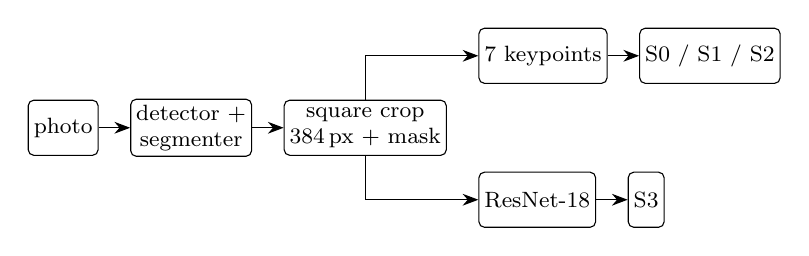
\begin{tikzpicture}[node distance=3mm and 4mm, every node/.style={font=\footnotesize},
  box/.style={draw, rounded corners=2pt, align=center, minimum height=7mm, inner sep=2pt},
  arr/.style={-{Stealth[length=2mm]}}]
\node[box] (img) {photo};
\node[box, right=of img] (seg) {detector +\\segmenter};
\node[box, right=of seg] (crop) {square crop\\384\,px + mask};
\node[box, above right=2mm and 4mm of crop] (kp) {7 keypoints};
\node[box, below right=2mm and 4mm of crop] (reg) {ResNet-18};
\node[box, right=of kp] (geo) {S0 / S1 / S2};
\node[box, right=of reg] (s3) {S3};
\draw[arr] (img) -- (seg);
\draw[arr] (seg) -- (crop);
\draw[arr] (crop) |- (kp);
\draw[arr] (crop) |- (reg);
\draw[arr] (kp) -- (geo);
\draw[arr] (reg) -- (s3);
\end{tikzpicture}
\caption{Pipeline. All strategies share the detector, crop and keypoints; S1 additionally uses the face mask.
Each outputs the reading $f$.}
\label{fig:pipeline}
\end{figure}

\section{Synthetic Data}\label{sec:data}
Every training image comes from the generator, so the reading and the camera pose are known exactly.

\textbf{Dial rendering.} Frontal faces are drawn at $1024\times1024$\,px with 2$\times$ supersampling: light
(80\,\%), dark (15\,\%) or coloured (5\,\%) faces; chrome, black or brass bezels; sweeps of 180, 240, 270
($p=0.5$) or 300 degrees centred on the top with $\pm10^\circ$ jitter; ranges 0--4, 0--10, 0--16, 0--100, 0--160
and $-1$--0 with major and minor ticks chosen so that 25, 50 and 75\,\% fall on ticks; numerals in six bundled
open fonts; optional coloured zones (30\,\%). Needles are tapered, arrow or counterweighted, in black, red or
white, never white on a light face nor black on a dark one. $f$ is uniform on $[0,1]$, with 5\,\% of dials
slightly outside (by up to 0.04).

\textbf{Pose and projection.} The face is the plane $z=0$ in millimetres (face radius 50\,mm). The camera has a
horizontal field of view in $[55^\circ,75^\circ]$; the dial is tilted by $\theta\sim U(0^\circ,65^\circ)$
about an in-plane axis with random azimuth, the camera is rolled by $\mathcal N(0,10^\circ)$, and the dial spans
25--70\,\% of the image width (images are $960\times720$ or $720\times960$). The plane $z$ is imaged by
$H_z = K\,[\,r_1\;\; r_2\;\; z\,r_3 + t\,]\,M$, where $M$ maps face pixels to millimetres. The needle lies on a
plane $z=\delta$ with $\delta$ between 2 and 5\,\% of the face radius, so the pivot and tip are projected with
$H_\delta$ and the scale points and face outline with $H_0$; this parallax is deliberate. The obliquity label is
computed from the pose, and poses whose label exceeds $65^\circ$ are resampled.

\textbf{Nuisances.} Applied after compositing, each with its own switch and random stream so that disabling one
leaves all other random draws unchanged: glare clipped to the face ($p=0.5$), shadows darkening a random
polygon by 20--60\,\% ($p=0.3$), low light with gamma 1.5--3, gain 0.3--0.7, Poisson shot noise and Gaussian
read noise ($p=0.3$), motion or defocus blur ($p=0.4$), and always colour jitter, white balance, vignetting and
JPEG quality 40--95. Backgrounds are crops of the 5,640 Describable Textures Dataset images~\cite{cimpoi2014}.
Fig.~\ref{fig:samples} shows examples.

\textbf{Splits.} 20,000 training and 2,000 validation images; the test set has 2,000 images stratified to 500
per obliquity bin. Generation depends only on the configuration, the split and the image index.

\begin{figure}[t]
\centering
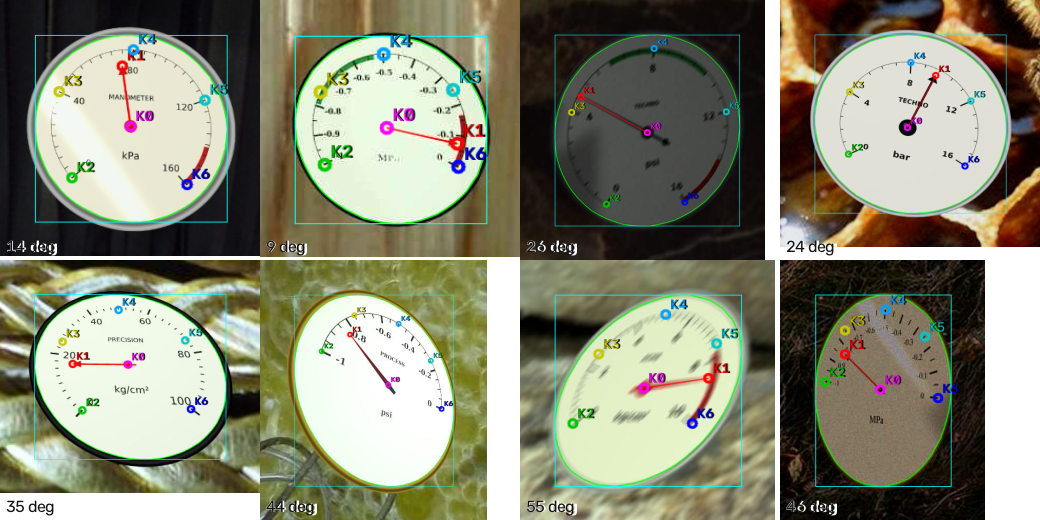
\includegraphics[width=\columnwidth]{figures/fig_samples.png}
\caption{Synthetic test images with ground-truth keypoints $K_0..K_6$ and obliquity: two per bin, including
glare, shadow, low light and blur.}
\label{fig:samples}
\end{figure}

\section{Experimental Setup}
\textbf{Training.} All models are trained on the synthetic training split only, on Kaggle with two NVIDIA T4
GPUs. The segmenter (YOLO26n-seg, pretrained) trained for 60 epochs at 640\,px, batch 32, with mosaic
augmentation and horizontal flips (6.8\,h). The keypoint model (YOLO26n-pose, pretrained) trained for 100 epochs
on 384\,px crops with $\pm8\,\%$ crop jitter, batch 64, rotation $\pm10^\circ$, no mosaic and \emph{no horizontal
flips}, since mirroring swaps the minimum and maximum and reverses the scale (4.7\,h). The regressor trained for
30 epochs with AdamW~\cite{loshchilov2019} (learning rate $3\times10^{-4}$, weight decay $10^{-4}$), a cosine
schedule~\cite{loshchilov2017}, batch 64, a Smooth-L1 loss with $\beta=0.02$ in units of $f$, and $\pm4\,\%$ crop
jitter without flips. Seeds are fixed. The models were trained on data generated before we fixed a renderer bug
that allowed black needles on dark faces (6.7\,\% of training images); the test set used below is generated with
the fix (Sec.~\ref{sec:discussion}).

\textbf{Experiments.} E1 applies S0--S2 to ground-truth keypoints (S1 uses the ground-truth face outline), then
adds Gaussian noise of $\sigma=1,2,4$\,px to all seven keypoints, with the same noise for every strategy on an
image. E2 runs the full trained system. E3 repeats E2 on real photographs and E4 retrains the keypoint and
regression models with one nuisance disabled at a time (Sec.~\ref{sec:real}).

\textbf{Metrics.} The mean (MAE) and median of the error in \%\,FS per obliquity bin and overall, the share of
images within 1 and 2.5\,\%\,FS, and the failure rate. Failures are excluded from the MAE and reported
separately. Each MAE has a 95\,\% percentile bootstrap interval from 1,000 resamples~\cite{efron1993}. Strategies are
compared on the images both read successfully, by the mean per-image difference in error with a paired
bootstrap interval.

\section{Results}\label{sec:results}

\subsection{E1: geometry with ground-truth keypoints}
Table~\ref{tab:e1} and Fig.~\ref{fig:e1} give the error with exact and noisy keypoints. Fig.~\ref{fig:rectify} shows one steep view before and after correction. Without correction the
error grows from 0.27 to 4.01\,\%\,FS between the lowest and highest bins. S1 and S2 reduce it to 0.36 and
0.35\,\%\,FS overall. On a separate 400-image test set with the needle on the face plane ($\delta=0$), S2 is
exact to numerical precision (MAE $2\times10^{-14}$\,\%\,FS), S1 reaches 0.064 and S0 1.64\,\%\,FS. With
parallax ($\delta>0$) the pivot leaves the dial plane, S2's assumption no longer holds, and its error grows with
obliquity to 0.72\,\%\,FS in the steepest bin, close to S1. On the same images S2 is still marginally better
than S1 with exact keypoints (paired difference $-0.009$\,\%\,FS, 95\,\% CI $[-0.013,-0.006]$), but S1 is
better as soon as keypoints are noisy ($+0.039$, $+0.086$ and $+0.150$\,\%\,FS in favour of S1 for
$\sigma=1,2,4$\,px, all intervals excluding zero). S2 also rejects more images through its linearity check
(1, 7, 38 and 251 of 2,000 for $\sigma=0,1,2,4$\,px), because five points leave no redundancy. In E1, S1 fits the exact face outline while S2
receives noisy keypoints, which favours S1 under noise.

\begin{table}[t]
\caption{E1: MAE (\%\,FS) with ground-truth keypoints plus Gaussian noise $\sigma$ (px); 500 images per bin,
95\,\% bootstrap interval on the overall MAE; failures out of 2,000.}
\label{tab:e1}
\centering
\footnotesize
\setlength{\tabcolsep}{3pt}
\begin{tabular}{@{}llrrrrlr@{}}
\toprule
 & $\sigma$ & 0--15$^\circ$ & 15--30$^\circ$ & 30--45$^\circ$ & 45--65$^\circ$ & overall & fail \\
\midrule
S0 & 0 & 0.27 & 0.68 & 1.87 & 4.01 & 1.71 [1.61, 1.81] & 0 \\
S1 & 0 & 0.09 & 0.21 & 0.39 & 0.74 & 0.36 [0.34, 0.37] & 0 \\
S2 & 0 & 0.08 & 0.21 & 0.38 & 0.72 & 0.35 [0.33, 0.36] & 1 \\
\midrule
S0 & 2 & 0.68 & 0.95 & 1.92 & 4.14 & 1.92 [1.83, 2.02] & 0 \\
S1 & 2 & 0.59 & 0.68 & 0.71 & 1.07 & 0.76 [0.73, 0.79] & 0 \\
S2 & 2 & 0.68 & 0.74 & 0.81 & 1.07 & 0.82 [0.79, 0.86] & 38 \\
\midrule
S0 & 4 & 1.24 & 1.42 & 2.33 & 4.21 & 2.30 [2.19, 2.41] & 0 \\
S1 & 4 & 1.22 & 1.23 & 1.37 & 1.73 & 1.39 [1.34, 1.45] & 0 \\
S2 & 4 & 1.31 & 1.29 & 1.45 & 1.56 & 1.40 [1.34, 1.45] & 251 \\
\bottomrule
\end{tabular}
\end{table}

\begin{figure}[t]
\centering
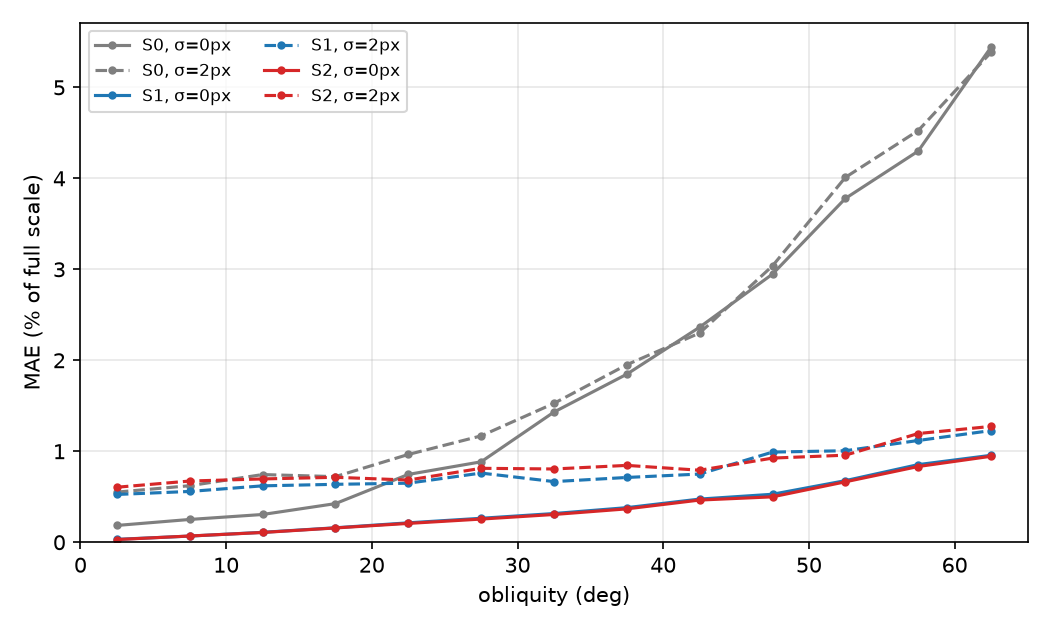
\includegraphics[width=\columnwidth]{figures/fig_e1.png}
\caption{E1: MAE in 5$^\circ$ obliquity bins with ground-truth keypoints ($\sigma=0$, solid) and with
$\sigma=2$\,px keypoint noise (dashed). S1 and S2 overlap.}
\label{fig:e1}
\end{figure}

\subsection{E2: full system on synthetic test images}
Table~\ref{tab:e2} and Fig.~\ref{fig:e2} report the trained system. The keypoint model's median error is 0.9\,\%
of the dial radius for the pivot, 1.6\,\% for the needle tip and 1.0--1.3\,\% for the scale points (95th
percentiles 2.4, 5.5 and 2.8--3.5\,\%). Without correction the error grows ninefold, from 0.45 to 4.16\,\%\,FS.
All three corrections stay at or below 1.12\,\%\,FS in every bin. Comparing strategies on the same images
(paired bootstrap, 1,000 resamples), S1 is more accurate than S2 by 0.037\,\%\,FS (95\,\% CI
$[0.024, 0.049]$), and S3 is less accurate than S1 by 0.150 ($[0.100, 0.207]$) and than S2 by 0.113
($[0.059, 0.175]$). These differences are statistically clear but small next to the uncorrected error; S3 needs
no keypoints.
S1 and S2 read 86 and 84\,\% of images within 1\,\%\,FS and 98\,\% within 2.5\,\%\,FS. The whole pipeline,
including all four strategies, ran at a median of 108\,ms per image on a laptop CPU (Apple M4).

\begin{table}[t]
\caption{E2: full system on the synthetic test set (n = 2,000). MAE in \%\,FS per obliquity bin, overall MAE
with 95\,\% bootstrap interval, share within 1 and 2.5\,\%\,FS, failures.}
\label{tab:e2}
\centering
\footnotesize
\setlength{\tabcolsep}{2.5pt}
\begin{tabular}{@{}lrrrrlrrr@{}}
\toprule
 & 0--15$^\circ$ & 15--30$^\circ$ & 30--45$^\circ$ & 45--65$^\circ$ & overall & $\le$1 & $\le$2.5 & fail \\
\midrule
S0 & 0.45 & 0.83 & 1.99 & 4.16 & 1.86 [1.75, 1.97] & 0.53 & 0.76 & 0 \\
S1 & 0.31 & 0.44 & 0.58 & 0.96 & 0.57 [0.53, 0.62] & 0.86 & 0.98 & 0 \\
S2 & 0.36 & 0.47 & 0.60 & 1.00 & 0.61 [0.57, 0.66] & 0.84 & 0.98 & 2 \\
S3 & 0.57 & 0.52 & 0.68 & 1.12 & 0.72 [0.65, 0.81] & 0.82 & 0.97 & 0 \\
\bottomrule
\end{tabular}
\end{table}

\begin{figure}[t]
\centering
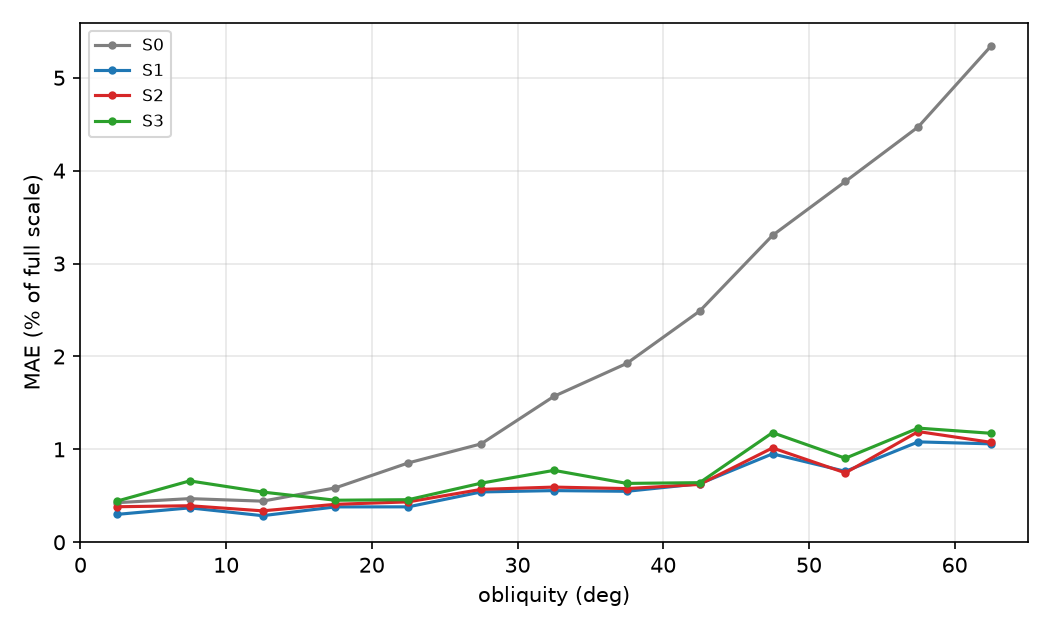
\includegraphics[width=\columnwidth]{figures/fig_e2.png}
\caption{E2: MAE of the trained system in 5$^\circ$ obliquity bins.}
\label{fig:e2}
\end{figure}

\begin{figure}[t]
\centering
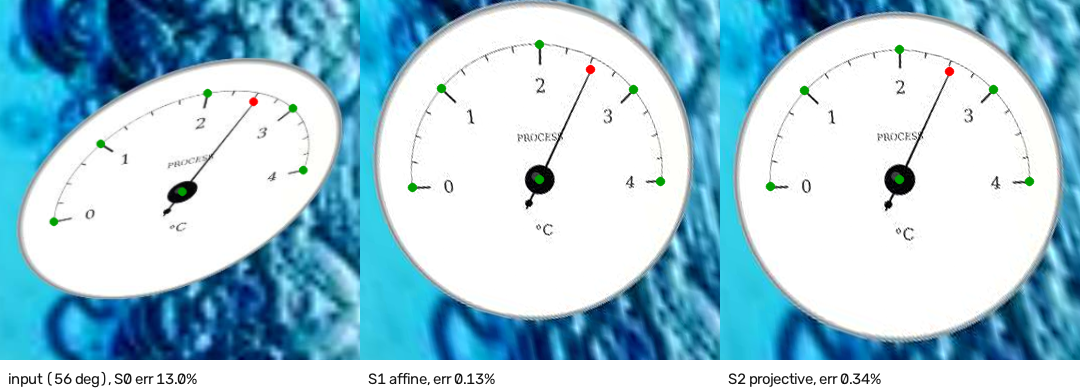
\includegraphics[width=\columnwidth]{figures/fig_rectify.png}
\caption{A 56$^\circ$ test view read with ground-truth keypoints. Measured in the image (S0) the reading is off
by 13.0\,\%\,FS; after affine (S1) or projective (S2) rectification the error is 0.13 and 0.34\,\%\,FS.}
\label{fig:rectify}
\end{figure}

\subsection{E3 and E4}\label{sec:real}
\textbf{Real test set (E3).} Photographs are taken with calibrated phones (checkerboard calibration~\cite{zhang2000})
and a 40\,mm ArUco marker~\cite{garridojurado2014} taped coplanar with the dial face; the obliquity label is
the angle between the marker normal, from planar pose estimation~\cite{collins2014}, and the camera ray through
the annotated pivot, with an ellipse-based fallback ($\theta\approx\arccos(b/a)$ of the face rim) when the marker
is unusable. On rendered marker scenes the marker-based label was within $1^\circ$ of the truth from 5 to
$65^\circ$. Keypoints are annotated in CVAT, and the reading of each gauge state is taken as the mean of two
independent readings of a frontal reference photograph. The real set is used for testing only.
The planned size is about 350 images with at least 50 per bin and at least five gauge faces.
\todo{E3 results: per-bin MAE table for S0--S3 from \texttt{eval.evaluate --split real}, number of images and
gauges actually collected, and the obliquity-label method counts (ArUco vs.\ ellipse).}

\textbf{Nuisance ablation (E4).} Five training sets differ from the default in exactly one setting (no glare,
no low light, no blur, no shadows, tilt limited to 0--10$^\circ$); each is image-for-image identical to the
default set except for that effect. \todo{E4 results: real-set MAE of the retrained keypoint and regression
models per ablation, or remove this paragraph if E4 is cut.}

\section{Discussion and Limitations}\label{sec:discussion}
\textbf{Why S2 does not beat S1.} Projective rectification is exact only if the pivot lies on the dial plane.
A real needle sits a few millimetres above the face, so the projected pivot is displaced from the image of the
dial centre by an amount that grows with obliquity. In our data this parallax costs S2 slightly more than the weak-perspective
approximation costs S1, and S1 also benefits from fitting the many points of the face outline rather than five
keypoints, which makes it less sensitive to keypoint errors. S2 also rejects more images under keypoint noise. A natural improvement is to fit the
conic to more scale points, which would give S2 redundancy.

\textbf{A data bug found by the evaluation.} A first E2 run showed 30 images with errors above 20\,\%\,FS for
every strategy, 29 of them black needles on dark faces, which are practically invisible. The renderer now forbids
this combination. The models in Table~\ref{tab:e2} were trained before the fix, so 6.7\,\% of their training
images had invisible needles; retraining on corrected data may lower the errors slightly.

\textbf{Limitations.} (i) All reported results are synthetic and the test set comes from the same generator as
the training data, so they measure in-distribution performance; the real-image evaluation (E3) is pending.
(ii) Each model was trained once, so the intervals do not include training variance. (iii) Obliquity is
limited to $65^\circ$ and dials are single-pointer and circular with linear scales. (iv) In E1, S1 uses the
exact face outline, which favours it under keypoint noise. (v) Our demonstration application optionally reads
the scale range from the printed numerals with OCR~\cite{du2020,rapidocr2021}; this is outside the evaluation,
and in informal tests on real photographs it often failed to recover the range.

\section{Conclusion}
On synthetic data with exact labels, camera tilt raises the error of an uncorrected keypoint-based reader about
ninefold between near-frontal and steep views, to about 4\,\%\,FS. Affine ellipse correction, projective
rectification and direct regression all keep the error near or below 1\,\%\,FS up to $65^\circ$, and the simple
affine correction is slightly more accurate than the projective one once needle parallax and keypoint errors are
present. Whether this ranking
holds on real photographs is the question the pending real-image evaluation will answer.

\section*{Acknowledgment}
This work was carried out as the course project of CS4231 Fundamentals of Computer Vision at RV University. We
thank Prof.\ Dr.~Ramakrishnan Varadharajan for his guidance.

\begin{thebibliography}{99}
\bibitem{alegria2000} F.~C. Alegria and A.~C. Serra, ``Automatic calibration of analog and digital measuring
instruments using computer vision,'' \emph{IEEE Trans. Instrum. Meas.}, vol.~49, no.~1, pp.~94--99, 2000.
\bibitem{howells2021} B.~Howells, J.~Charles, and R.~Cipolla, ``Real-time analogue gauge transcription on mobile
phone,'' in \emph{Proc. IEEE/CVF CVPR Workshops}, 2021, pp.~2369--2377.
\bibitem{leonalcazar2024} J.~Leon-Alcazar, Y.~Alnumay, C.~Zheng, H.~Trigui, S.~Patel, and B.~Ghanem, ``Learning
to read analog gauges from synthetic data,'' in \emph{Proc. IEEE/CVF WACV}, 2024, pp.~8616--8625.
\bibitem{reitsma2024} M.~Reitsma, J.~Keller, K.~Blomqvist, and R.~Siegwart, ``Under pressure: Learning-based
analog gauge reading in the wild,'' in \emph{Proc. IEEE ICRA}, 2024; arXiv:2404.08785.
\bibitem{tobin2017} J.~Tobin, R.~Fong, A.~Ray, J.~Schneider, W.~Zaremba, and P.~Abbeel, ``Domain randomization
for transferring deep neural networks from simulation to the real world,'' arXiv:1703.06907, 2017.
\bibitem{hartley2004} R.~Hartley and A.~Zisserman, \emph{Multiple View Geometry in Computer Vision}, 2nd~ed.
Cambridge, U.K.: Cambridge Univ. Press, 2004.
\bibitem{bradski2000} G.~Bradski, ``The OpenCV Library,'' \emph{Dr. Dobb's J. Softw. Tools}, 2000.
\bibitem{jocher2026} G.~Jocher, J.~Qiu, M.~Liu, S.~Lyu, F.~C. Akyon, and M.~E. Kalfaoglu, ``Ultralytics YOLO26:
Unified real-time end-to-end vision models,'' arXiv:2606.03748, 2026.
\bibitem{he2016} K.~He, X.~Zhang, S.~Ren, and J.~Sun, ``Deep residual learning for image recognition,'' in
\emph{Proc. IEEE CVPR}, 2016, pp.~770--778.
\bibitem{deng2009} J.~Deng, W.~Dong, R.~Socher, L.-J. Li, K.~Li, and L.~Fei-Fei, ``ImageNet: A large-scale
hierarchical image database,'' in \emph{Proc. IEEE CVPR}, 2009, pp.~248--255.
\bibitem{cimpoi2014} M.~Cimpoi, S.~Maji, I.~Kokkinos, S.~Mohamed, and A.~Vedaldi, ``Describing textures in the
wild,'' in \emph{Proc. IEEE CVPR}, 2014, pp.~3606--3613.
\bibitem{loshchilov2019} I.~Loshchilov and F.~Hutter, ``Decoupled weight decay regularization,'' in
\emph{Proc. ICLR}, 2019.
\bibitem{loshchilov2017} I.~Loshchilov and F.~Hutter, ``SGDR: Stochastic gradient descent with warm restarts,''
in \emph{Proc. ICLR}, 2017.
\bibitem{efron1993} B.~Efron and R.~J. Tibshirani, \emph{An Introduction to the Bootstrap}. New York, NY, USA:
Chapman \& Hall, 1993.
\bibitem{zhang2000} Z.~Zhang, ``A flexible new technique for camera calibration,'' \emph{IEEE Trans. Pattern
Anal. Mach. Intell.}, vol.~22, no.~11, pp.~1330--1334, 2000.
\bibitem{garridojurado2014} S.~Garrido-Jurado, R.~Mu\~noz-Salinas, F.~J. Madrid-Cuevas, and M.~J.
Mar\'in-Jim\'enez, ``Automatic generation and detection of highly reliable fiducial markers under occlusion,''
\emph{Pattern Recognit.}, vol.~47, no.~6, pp.~2280--2292, 2014.
\bibitem{collins2014} T.~Collins and A.~Bartoli, ``Infinitesimal plane-based pose estimation,'' \emph{Int. J.
Comput. Vis.}, vol.~109, no.~3, pp.~252--286, 2014.
\bibitem{du2020} Y.~Du \emph{et al.}, ``PP-OCR: A practical ultra lightweight OCR system,'' arXiv:2009.09941,
2020.
\bibitem{rapidocr2021} RapidAI Team, ``RapidOCR: OCR toolbox,'' 2021. [Online]. Available:
\url{https://github.com/RapidAI/RapidOCR}
\end{thebibliography}

\end{document}
